\documentclass[a4paper,11pt]{book}
\usepackage{latexsym}
\usepackage[MeX]{polski}
\usepackage[utf8]{inputenc}
\usepackage{url}
\usepackage{rotating}
\usepackage{listings}
\usepackage{color}
\usepackage[pdftex]{graphicx}
\usepackage{footnote}
\usepackage{packages/zmienne}	
\usepackage{packages/strona_tytulowa}
\usepackage{packages/oswiadczenie}
\usepackage{packages/karta_pracy}
\usepackage{extsizes}							%wiecej rozmiaróww czcionek
\usepackage[a4paper,left=3.5cm,right=2.5cm,top=2.5cm,bottom=2.5cm]{geometry}
\usepackage{tocloft}								% format spisu treści
\usepackage{array}								% lepiej wyglądające tabelki
\usepackage[format=hang,labelsep=period,labelfont={bf,small},textfont=small]{caption}
\usepackage{floatflt}							% ładniejsze opisywanie obrazków tekstem
\usepackage{subfig}								% możliwość wstawiania figur w kolumnach
\usepackage{graphicx}							% do obsługi grafiki
\usepackage{here}									% wymuszanie położenia figury w danym miejscu
\usepackage{url}									% adresy internetowe
\usepackage{enumerate}							% modyfikowanie list wyliczeniowych np \begin{enumerate}[(a)]...
\usepackage{multirow}							% do tabel
\usepackage{slantsc}
\usepackage[T1]{fontenc}
\usepackage{lmodern}\normalfont %to load T1lmr.fd
\usepackage{algorithm}
\usepackage{algorithmic}
\usepackage{amsmath}
\usepackage{amssymb}
\usepackage[pdftex,usenames,dvipsnames]{color}

\usepackage{dashrule}
\usepackage{fancyhdr} 							% do stopki i nagłówka
\usepackage{calc}
\usepackage{packages/zmienne}				
\usepackage{longtable}							% do podziału tabel na wiele stron

\usepackage{indentfirst}
\floatname{algorithm}{Algorytm}
\usepackage[section]{placeins}
\usepackage{nomencl}
\makenomenclature
\usepackage{makeidx}
\makeindex
\renewcommand{\nomname}{Spis ważniejszych symboli}

\definecolor{mygreen}{rgb}{0,0.6,0}
\definecolor{mygray}{rgb}{0.5,0.5,0.5}
\definecolor{mymauve}{rgb}{0.58,0,0.82}

\lstset{ %
	backgroundcolor=\color{white},  
	basicstyle=\footnotesize,        % the size of the fonts that are used for the code
	breakatwhitespace=true,          % sets if automatic breaks should only happen at whitespace
	breaklines=false,                % sets automatic line breaking
	captionpos=b,                    % sets the caption-position to bottom
	commentstyle=\color{mygreen},    % comment style
	deletekeywords={},            	 % if you want to delete keywords from the given language
	escapeinside={\%*}{*)},          % if you want to add LaTeX within your code
	extendedchars=true,              % lets you use non-ASCII characters; for 8-bits encodings only, does not work with UTF-8
	frame=single,                    % adds a frame around the code
	keepspaces=true,                 % keeps spaces in text, useful for keeping indentation of code (possibly needs columns=flexible)
	keywordstyle=\color{blue},       % keyword style
	language=Java,                 	 % the language of the code
	otherkeywords={@Data, @NoArgsConstructor, @Entity, @NamedQueries, @Table, @NamedQuery},           	 % if you want to add more keywords to the set
	numbers=left,                    % where to put the line-numbers; possible values are (none, left, right)
	numbersep=-10pt,                 % how far the line-numbers are from the code
	numberstyle=\tiny\color{mygray}, % the style that is used for the line-numbers
	rulecolor=\color{black},         % if not set, the frame-color may be changed on line-breaks within not-black text (e.g. comments (green here))
	showspaces=false,                % show spaces everywhere adding particular underscores; it overrides 'showstringspaces'
	showstringspaces=false,          % underline spaces within strings only
	showtabs=false,                  % show tabs within strings adding particular underscores
	stepnumber=1,                    % the step between two line-numbers. If it's 1, each line will be numbered
	stringstyle=\color{mymauve},     % string literal style
	tabsize=2,                       % sets default tabsize to 2 spaces
	title=\lstname                   % show the filename of files included with \lstinputlisting; also try caption instead of title
}

\newenvironment{italicquote}
{\begin{quote}\itshape}
{\end{quote}}

\author{Piotr~Joński}
\kierunek{Informatyka}
\specjalnosc{Sieciowe systemy informatyczne}
\grupa{431 IDZ}
\title{System zarządzania projektami dedykowany metodyce Scrum}
\tytulAngielski{Project management system dedicated to Scrum methodology}
\uczelnia{Uniwersytet Zielonogórski}
\wydzial{Wydział Informatyki, Elektrotechniki i Automatyki}
\praca{Praca dyplomowa}
\promotor{dr inż. Andrzej~Marciniak}
\konsultant{} 
\miasto{Zielona Góra}
\miesiac{luty}
\rok{2016}
\dzien{10} 			
\mm{02}
\podjecieTematu{18.03.2015} 


\celPracy{Celem pracy jest wytworzenie systemu, który będzie umożliwiał intuicyjne zarządzanie projektem.}

\numZakres{4}

\zakresI{Opracowanie wymagań funkcjonalnych i niefunkcjonalnych dla projektowanego systemu,}
\zakresII{Wytworzenie projektu i implementacja systemu,}
\zakresIII{Wykonanie testów aplikacji,}
\zakresIV{Wytworzenie dokumentacji i zredagowanie części opisowej pracy.}

\pagenumbering{roman}

\makeatletter
    \def\numberline#1{\hb@xt@\@tempdima{#1.\hfil}}                      %kropki w spisie treœci
    \renewcommand*\@seccntformat[1]{\csname the#1\endcsname.\enspace}   %kropki w treści dokumentu
\makeatother

\makeatother
% ------------------------------------------------------------------------
% Definicje
% ------------------------------------------------------------------------
\def\nonumsection#1{%
    \section*{#1}%
    \addcontentsline{toc}{section}{#1}%
    }
\def\nonumsubsection#1{%
    \subsection*{#1}%
    \addcontentsline{toc}{subsection}{#1}%
    }
\reversemarginpar %umieszcza notki po lewej stronie, czyli tam gdzie jest wiêcej miejsca
\def\notka#1{%
    \marginpar{\footnotesize{#1}}%
    }
%\def\mathcal#1{%
%    \mathscr{#1}%
%    }

\newcommand{\myemptypage}{ \newpage  \thispagestyle{empty}~\newpage}

%-------------------------------------------------------------------------
% stopka i nagłówek
%-------------------------------------------------------------------------
\setlength{\headheight}{15pt}

\pagestyle{fancy}
\renewcommand{\chaptermark}[1]{\markboth{#1}{}}
\renewcommand{\sectionmark}[1]{\markright{#1}{}}

\fancyhf{}
\fancyhead[LE,RO]{\thepage}
\fancyhead[RE]{\textit{\nouppercase{\leftmark}}}
\fancyhead[LO]{\textit{\nouppercase{\rightmark}}}

\fancypagestyle{plain}{ %
\fancyhf{}
\renewcommand{\headrulewidth}{0pt}
\renewcommand{\footrulewidth}{0pt}}

% ------------------------------------------------------------------------
% Inne
% ------------------------------------------------------------------------
\frenchspacing
\setlength{\parskip}{3pt}           	%odstêp pomiêdzy akapitami
%\linespread{1.49}                    	%odstêp pomiêdzy liniami (interlinia)
\setcounter{tocdepth}{3}
\setcounter{secnumdepth}{3}


% ------------------------------------------------------------------------
% Polskie podpisy
% ------------------------------------------------------------------------
\renewcommand{\figurename}{Rys.}
\renewcommand{\tablename}{Tab.}

% ------------------------------------------------------------------------
% Bibliografia
% ------------------------------------------------------------------------
\bibliographystyle{unsrt}					% kolejnoœæ wed³óg u¿ycia
%\bibliographystyle{plain}					% kolejnoϾ alfabetyczna



%==========================================================================================
% Deklaracja fontow kapitalikowych z kodowaniem T1
%==========================================================================================
\DeclareFontShape{T1}{lmr}{bx}{sc} { <-> ssub * cmr/bx/sc }{}
\DeclareFontShape{T1}{lmr}{bx}{scit}{<-> ssub * cmr/bx/scsl}{}
%==========================================================================================
% Inne deklaracje
%==========================================================================================
\renewcommand*{\lstlistlistingname}{Spis listingów}
\newcommand{\specialcell}[2][c]{%
		\begin{tabular}[#1]{@{}c@{}}#2\end{tabular}}
	
	

\begin{document}

\newgeometry{left=2cm, right=2cm, top=1cm,bottom=2cm,headsep=1cm}
\thispagestyle{empty}
\kartapracy
\myemptypage

\newgeometry{left=3.5cm,right=2.5cm,top=2.5cm,bottom=2.5cm}	
\linespread{1.49}
\thispagestyle{empty}
\stronatytulowa

\normalsize
\oswiadczenie
\newpage

\subsection*{Streszczenie}


CO TU DAĆ?


\vspace{1cm}
\noindent\textbf{słowa kluczowe:} praca dyplomowa, skład komputerowy, formatowanie dokumentu.
\myemptypage

%========================================================================================
% Spis tresci, spis tabel i~rysunków
%========================================================================================
%spis tresci
\tableofcontents
\newpage
%\myemptypage
%spis rysunków
\listoffigures
\newpage
%\myemptypage
%spis tabel
\listoftables
\newpage
%\myemptypage
\lstlistoflistings
\newpage

%========================================================================================
% Licznik Stron
%========================================================================================
\newcounter{licznikStron}
\setcounter{licznikStron}{\value{page}}
\setcounter{licznikStron}{1}
\pagenumbering{arabic}
\setcounter{page}{\value{licznikStron}}

%Rozdziały
\chapter{Wstęp}
\section{Wprowadzenie i przegląd literatury}

Co tu dać?

\section{Cel i zakres pracy}
Celem pracy było wytworzenie systemu do zarządzania projektami dedykowanego metody Scrum. Obecnie na rynku jest wiele zarówno darmowych jak i płatnych narzędzi, które oferują możliwość prowadzenia projektów rożnymi metodykami. W zakres pracy wchodzą:
\begin{enumerate}
	\item zapoznanie się z literaturą tematu,
	\item opracowanie założeń projektu,
	\item spis wymagań funkcjonalnych i niefunkcjonalnych systemu,
	\item implementacja wszystkich funkcjonalności oraz usunięcie powstałych błędów,
	\item przetestowanie systemu ,
	\item wytworzenie części opisowej pracy.
	
\end{enumerate}


\section{Struktura pracy}
Opis rozdziałów zostanie uzupełniony na końcu pracyitemize
\chapter{Wprowadzenie}
\section{Szkic problemu}

Szybki rozwój w dziedzinie informatyki spowodował wzrost zapotrzebowania na systemy, które pomogłyby rozwiązywać problemy kwestii organizacyjnej projektów. W dzisiejszych czasach zarządzanie projektami jest szerokim zagadnieniem, a na jego temat powstało wiele publikacji. Autorzy proponują takie rozwiązania dot. zarządzania projektami jak:
\begin{enumerate}
	\item scrum,
	\item lean Softrware Development,
	\item feature Driven Development,
	\item test Driven Develipment.
\end{enumerate}

Nie jest to wyczerpująca lista metodyk - istnieje wiele innych metod tworzenia oprogramowania, jednak opis wszystkich wykracza po za zakres tej pracy. W mojej pracy dyplomowej poruszam temat systemu do zarządzania projektami, który jest dedykowany metodyce Scrum. Nie bez powodu wybrana została właśnie ta zwinna metodyka - jest to na chwilę obecną najbardziej popularna metoda wytwarzania oprogramowania, a umiejętności pracy wraz z nią są pożądane przez większość pracodawców na całym świecie.

Scrum jest zwinną metodyką wytwarzania oprogramowania, której początki sięgają połowy lat 80. Aby prawidłowo przedstawić omawiany temat należy zapoznać się z pojęciami, które są nieodłącznym elementem tej metody:
\begin{enumerate}
	\item \textbf{product owner} - osoba odpowiedzialna za projekt,
	\item \textbf{scrum master} - osoba, która pomaga zespołowi w organizacji czasu pracy a także rozwiązuje powstałe problemu,
	\item \textbf{zespół developerski} - zespół programistów wspólnie pracujący nad wytworzeniem produktu,
	\item \textbf{backlog produktu} - jest to zbiór zadań / funkcjonalności wchodzące w skład wytwarzanego projektu,
	\item \textbf{sprint} - interwały czasowe, w których realizowane są zadania. Bezpośrednio przed każdym sprintem występuje planowanie, czyli wybieranie funkcjonalności do zrealizowania w danym sprincie. Bezpośrednio po sprincie powinna wystąpić retrospektywa oraz demo produktu, które jest często pomijane przez wiele zespołów,
	\item \textbf{story} - najmniejsza jednostka podlegająca ocenie (wg. wybranej przez zespół skali). 
	\item \textbf{task} - zadania, które mogą być powiązane bezpośrednio ze story lub projektem.
	\item \textbf{retrospektywa} - wydarzenie, które ma miejsce na koniec sprintu. W tym momencie zespół developerski spisuje wszystkie wady i zalety minionego sprintu oraz wspólnie z scrum masterem starają się rozwiązać zaistniałe problemy.
\end{enumerate} 

\section{Przegląd dostępnych narzędzi}
Wytwarzając ten system skupiłem się, aby wpasował się on w wybraną przeze mnie metodykę oraz rozwiązywał szereg mankamentów, które napotkałem podczas korzystania z obecnych już rozwiązań. W celu lepszego zrozumienia problemów postanowiłem opisać kilka z nich.

Pierwszym i niewątpliwie największym problemem tego typu systemów jest to, że są one płatne, przez co nie wszystkich na nie stać. Niektóre są darmowe, lecz tylko dla projektów typu open source, co nie sprawdza się podczas pracy nad wspólnymi projektami w firmie lub np. pracą dyplomową.

Kolejną wadą jest to, że nie są one proste w instalacji. Często występują jako potężne programy, przez co nie można ich bezpłatnie hostować w chmurze gdyż potrzebują dużo płatnych zasobów. 

Ostatnim, jednak nie mniej ważnym problemem jest ich czytelność. Oferują one szereg zbędnej zwykłemu użytkownikowi - programiście - funkcjonalności, która jest przydatna tylko w określonych warunkach. Taki ogrom zakładek i okienek powoduje często zamęt i niezrozumienie wśród programistów.


Poniższa tabela przedstawia 
------------------------------------------------------------------------------------------------------

Celem pracy było wytworzenie systemu do zarządzania projektami dedykowanego metody Scrum. Obecnie na rynku jest wiele zarówno darmowych jak i płatnych narzędzi, które oferują możliwość prowadzenia projektów rożnymi metodykami. Mają one jednak pewne wady:
\begin{enumerate}
	\item Darmowe narzędzia nie są wspierane, przez co ich rozwój stanął w miejscu wiele lat temu
	\item Część z nich jest darmowa tylko dla 10 użytkowników, co powoduje, że nie są przydatne w większych firmach
	\item Większość jest darmowa tylko dla open source, co wyklucza możliwość użycia ich w firmie
	\item Posiadają przerost formy nad treścią - docelowy użytkownik - programista musi przedzierać się przez gąszcz funkcjonalności oraz poświęcać czas na system, zamiast na swoją pracę
\end{enumerate}

Wytworzony przeze mnie system ma na celu sprostać wadom obecnego oprogramowania oraz spełniać następujące wymagania:
\begin{enumerate}
	\item Łatwość instalacji - do tego celu zostało wykorzystane oprogramowanie docker, które wspiera szybkie wytwarzanie oprogramowania
	\item Przejrzysty interfejs użytkownika - został osiągnięty dzięki open sourcowej bibliotece PrimeFaces
	\item Bez zbędnej funkcjonalności - zostały zaimplementowane tylko obligatoryjne funkcje tego typu systemu oraz niewielka ilość udogodnień
\end{enumerate}


\chapter{Dokumentacja projektowa}

\section{Architektura systemu}
Wytworzony w ramach pracy system jest aplikacją webową, która korzysta z bazy danych do odczytu i zapisu niezbędnych informacji. Z systemu będą korzystać cztery, wcześniej omówione, rodzaje użytkowników poprzez interfejs WWW. Dodatkowo system został zaprojektowany w taki sposób, aby była możliwość rozbudowy o dodatkowe zdalne aplikacje klienckie umożliwiające komunikację z systemem. System wraz z bazą danych znajdują się w kontenerze Dockera.

Jak wiadomo, połączenie ze zdalnymi klientami nie jest gwarantowane, co skłania do zastosowania mechanizmu komunikacji Java Message Service (JMS). Jednak pomimo, że połączenie nie jest ani stabilne, ani nawet w ogóle nie wiadomo czy zostało nawiązane, zależy nam, aby informować użytkowników o różnego rodzaju błędach, lub przesyłać im dane na bieżąco. Co prawda JMS umożliwia realizację tego zadania lecz do komunikacji z samodzielną aplikacją zostały udostępnione inne ścieżki komunikacji. 

Pierwsza z nich to warstwa usługi REST. Dzięki takiemu rozwiązaniu z aplikacją może komunikować się dowolny system niezależnie od tego w jakim języku został napisany. Warstwa ta nie została zaimplementowana w całości, lecz jedynie jako fragment funkcjonalności w celu zobrazowania komunikacji ze zdalnymi klientami.

Kolejna ścieżka komunikacji to zdalny interfejs komponentu EJB (Enterprise JavaBean). Mechanizm ten wprowadza możliwość komunikacji asynchronicznej z aplikacją. Jest on jednak ograniczony tylko do klientów napisanych w języku Java.

Wyżej wymienione rozwiązania stanowią warstwę do komunikacji z aplikacjami klienckimi. Kolejnym krokiem było zaprojektowanie warstwy do komunikacji z klientem WWW. Co prawda warstwa REST spełniałaby swoje wymagania, lecz w tym celu posłużymy się, specjalnie zaprojektowaną do tego rodzaju zadań, technologią JavaServer Faces (JSF). Rozwiązanie to pozwoli nam zaimplementować dodatkową warstwę, dedykowaną specjalnie dla interfejsu WWW. Warstwa ta to tzw. komponenty Java Beans zwane również Backing Beans (BB). Rysunek \ref{fig:diagsys} przedstawia diagram systemowy aplikacji:

\begin{figure}[h!]
	\centering
	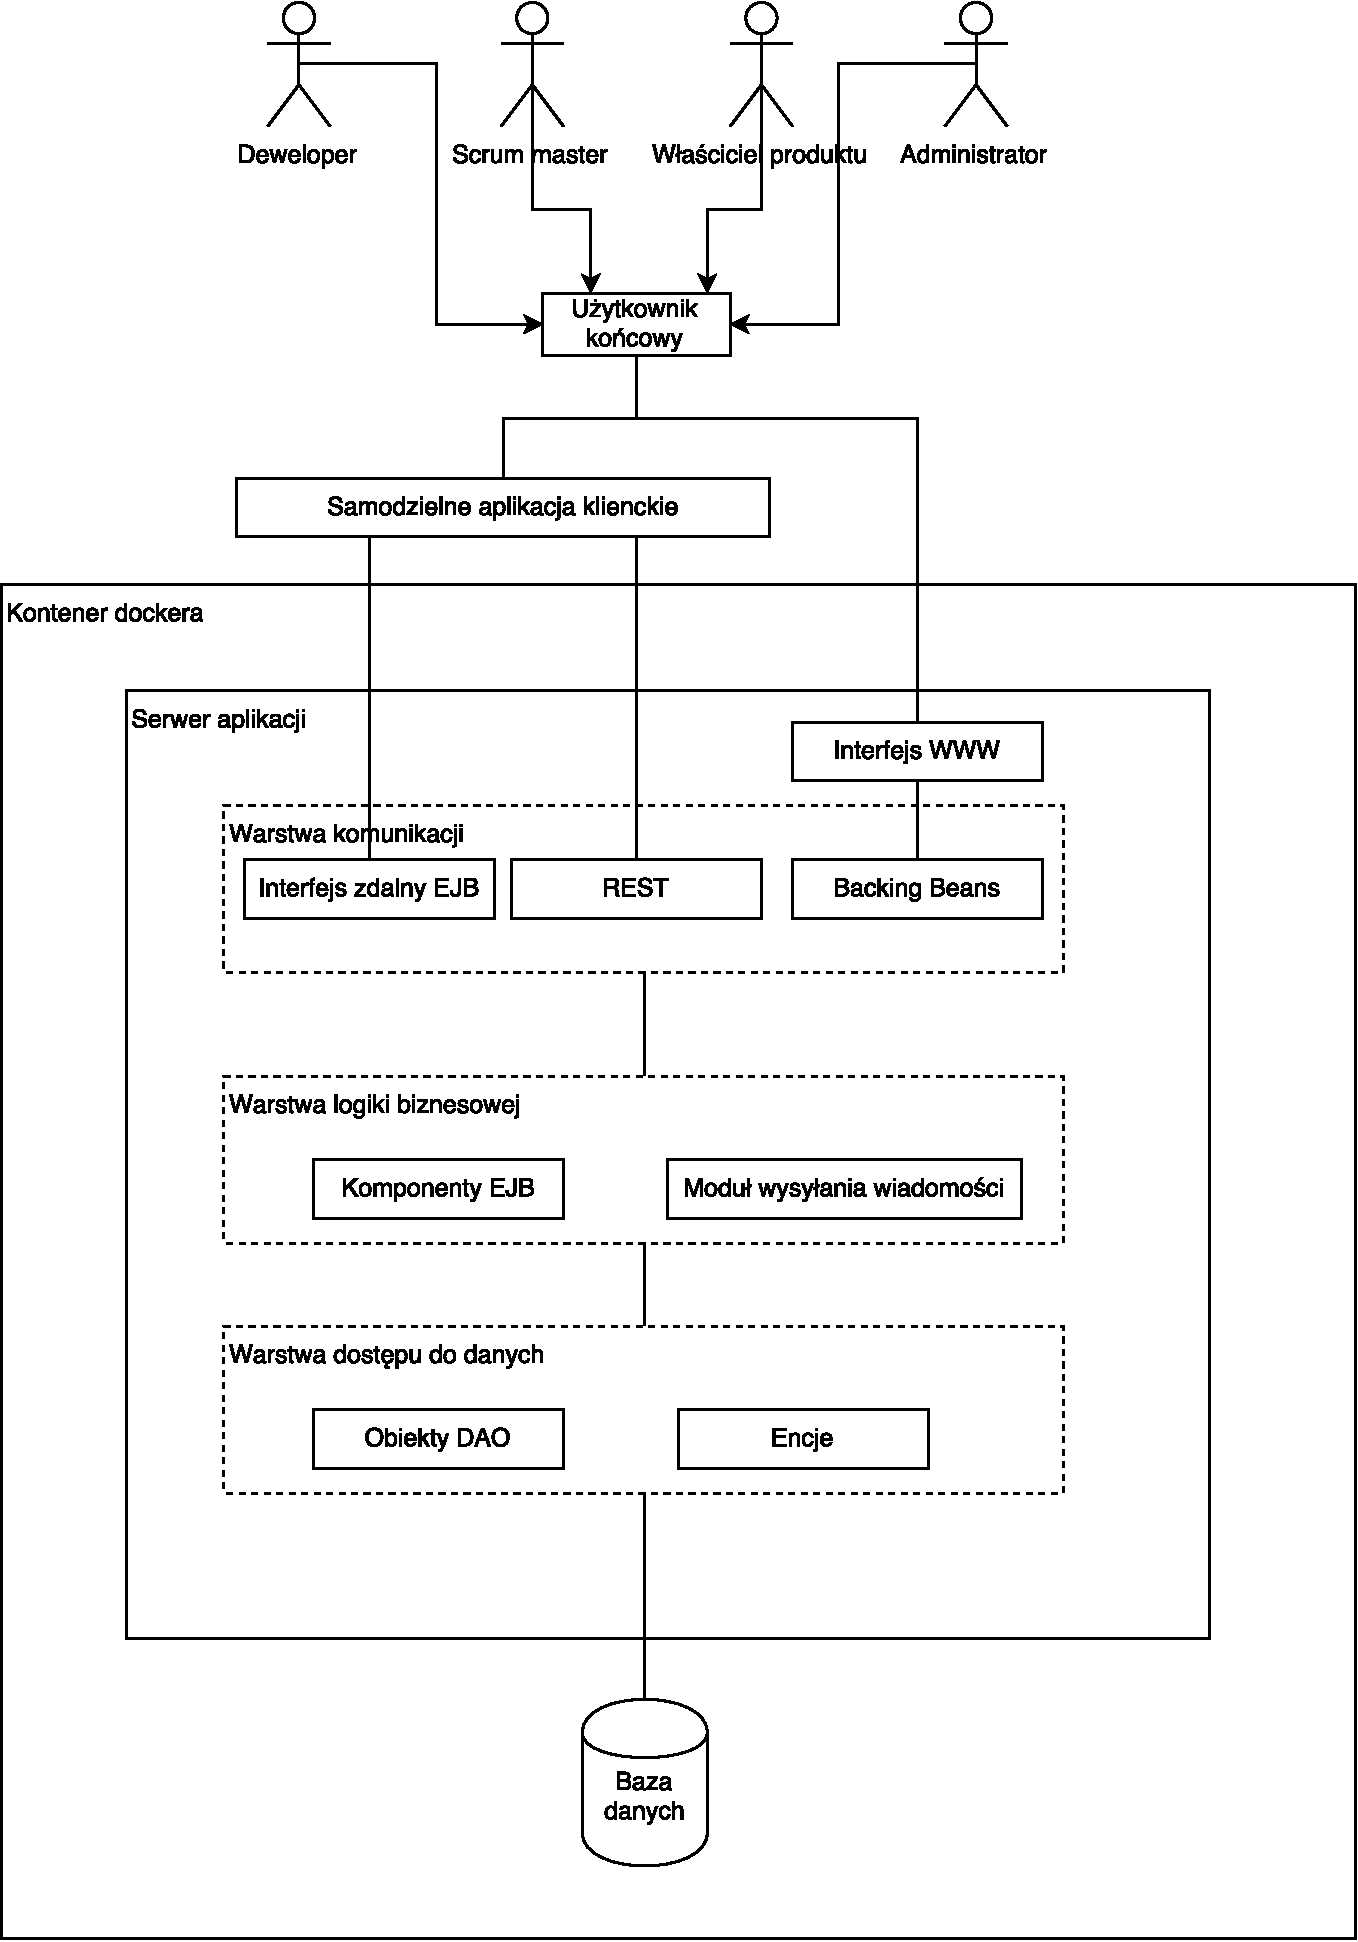
\includegraphics[width=13.5cm]{rysunki/diagsys.pdf}	
	\caption{Diagram systemowy aplikacji}
	\label{fig:diagsys}
\end{figure}

Jak wiadomo, interfejsy graficzne, a co za tym idzie – sposób ich obsługi będą się różniły w zależności od klienta. Najważniejszą różnicą będzie sposób walidacji danych oraz obsługi błędów. W samodzielnej aplikacji klienckiej walidacja danych oraz obsługa błędów powinna wystąpić możliwie szybko, aby nie generować zbędnego ruchu sieciowego. Jeżeli w trakcie przetwarzania żądania wystąpią jakiekolwiek błędy, to powinny one zostać zamienione na wyjątki aplikacji oraz przekazane do klienta. Również w aplikacji WWW walidacja danych wejściowych powinna znajdywać się na poziomie klienta. Jednak nie można wykluczyć sytuacji, w której błędy pojawią się po stronie serwera nawet po poprawnej walidacji danych. Z tego względu błędy powinny być konwertowane po stronie serwera (przez dodatkową warstwę obsługi JSF) na obiekty typu FaceMessage i dodawane bezpośrednio do kontekstu aplikacji WWW. 

Wymagania odnośnie walidacji oraz obsługi błędów mogą skłaniać do wprowadzenia dodatkowej warstwy w architekturze systemu. Nie mniej jednak taka warstwa nie została wprowadzona, gdyż spowodowało by to nadmierny przyrost klas oraz niepotrzebne uogólnienie systemu. Zamiast tego logika biznesowa generuje wyjątki aplikacji, gdy zajdzie taka potrzeba oraz przekazuje je warstwie wyżej lub klientom, które wywołują dane komponenty logiki biznesowej. Oznacza to tyle, że obsługa błędów aplikacji w samodzielnej aplikacji Javy powinna być zaimplementowana po stronie samej aplikacji, natomiast interfejs WWW posiada dodatkową warstwę w postaci komponentów JavaBeans, które takową obsługę zapewnią. 

\subsection{Identyfikacja komponentów biznesowych}
W oparciu o artefakty metodyki Scrum oraz wymagania funkcjonalne z systemu wyłaniają się następujące komponenty biznesowe:

\textit{Deweloper} -- użytkownik aplikacji, może przeglądać oraz modyfikować \textit{zadania} w \textit{projektach}, do których należy.

\textit{Scrum master} -- użytkownik aplikacji, jest przypisany do jednego lub wielu \textit{zespołów}.

\textit{Właściciel produktu} -- użytkownik aplikacji, jest przypisany tylko do jednego \textit{projektu}.

\textit{Administrator} -- użytkownik aplikacji, zarządza całym systemem. Może tworzyć nowe \textit{projekty} oraz \textit{zespoły}.

\textit{Zespół} -- zbiór \textit{deweloperów}, może być powiązany z \textit{projektem}.

\textit{Projekt} -- zbiór \textit{zadań}, posiada \textit{właściciela produktu}.

\textit{Sprint} -- jest tworzone przez  \textit{scrum mastera}. Posiada story.

\textit{Story} -- jest agregatem \textit{zadań}.

\textit{Backlog} -- przynależy do \textit{projektu}, posiada \textit{zadania}.

\textit{Zadanie} -- jest tworzone przez \textit{użytkowników}.


Należy wspomnieć, iż jest to częściowy opis obiektów biznesowych, który ma na celu zobrazowanie procesu powstawania aplikacji. Wyczerpujący opis tych obiektów byłby zbyt rozległy i nie jest on meritum części opisowej pracy. Aby zobrazować wpływ poszczególnych jednostek biznesowych oraz ich wzajemne relacje należy przedstawić ich diagram UML:
\begin{figure}[h!]
	\centering
	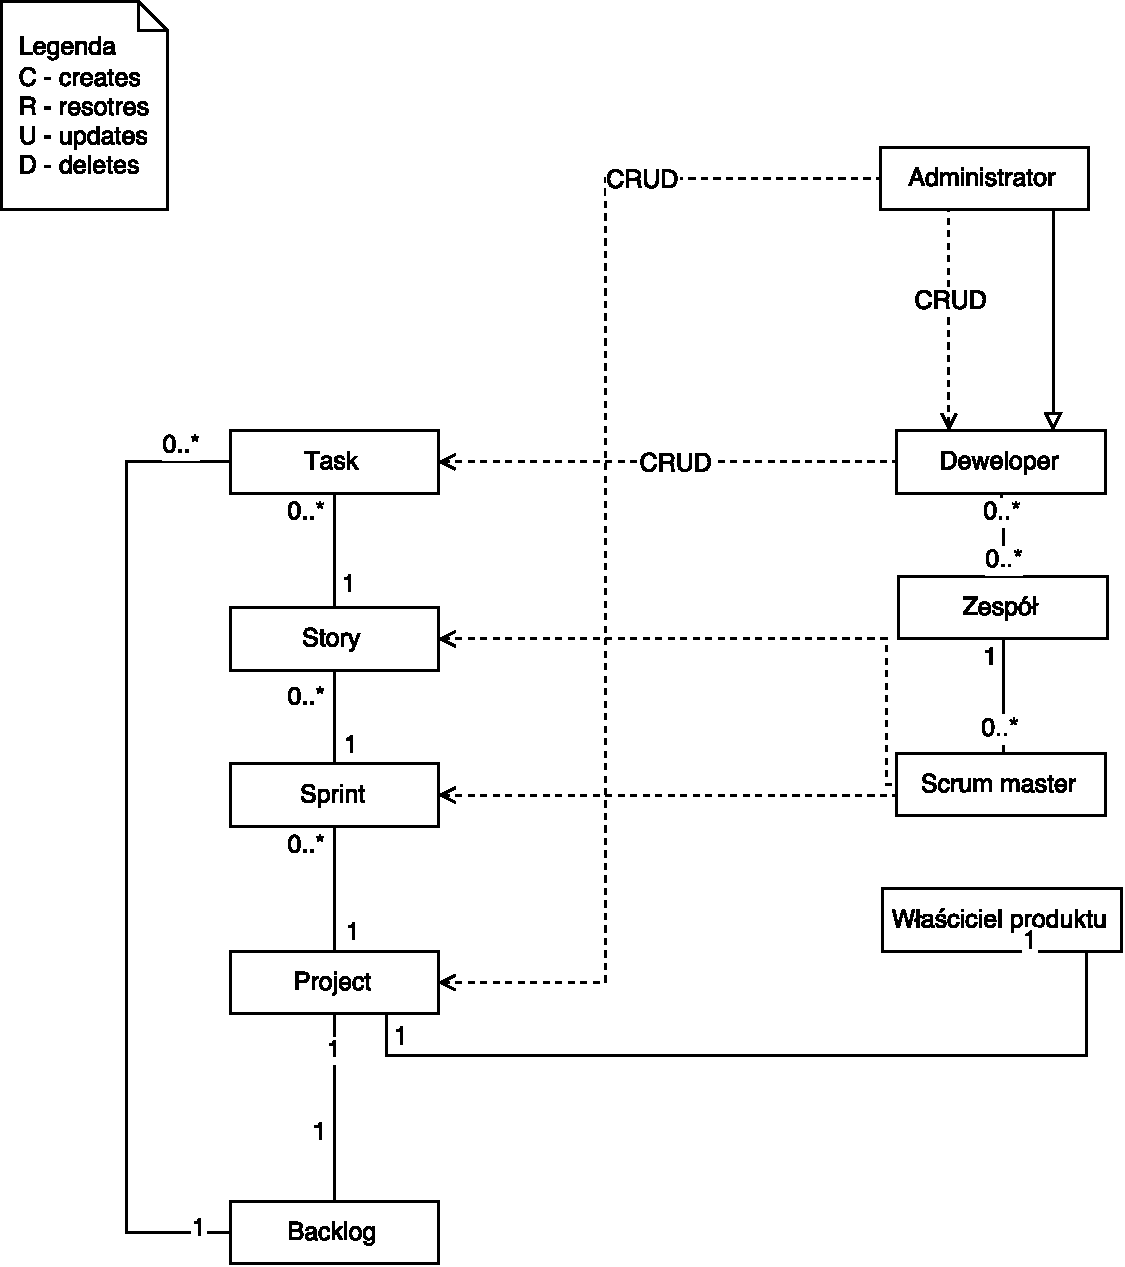
\includegraphics[width=15cm]{rysunki/diaguml.pdf}	
	\caption{Diagram jednostek biznesowych}
	\label{fig:diaguml}
\end{figure}

\section{Struktura projektu}
W poprzedniej sekcji została opisana ogólna architektura systemu umożliwiająca pogląd na całą aplikację. Teraz zostaną opisane wybrane komponenty. Zanim jednak to zrobimy zostanie przedstawiony bardziej szczegółowy diagram jednostek biznesowych, który uwzględnia funkcje, jakie można wykonywać w systemie. Diagram powstał w oparciu o wymagania funkcjonalne, które szczegółowo opisują, co dany użytkownik może robić, oraz o identyfikację komponentów biznesowych omówionych wcześniej. Także i tutaj należy zwrócić uwagę, iż nie jest to wyczerpujący diagram klas opracowanych w systemie:
\begin{figure}[h!]
	\centering
	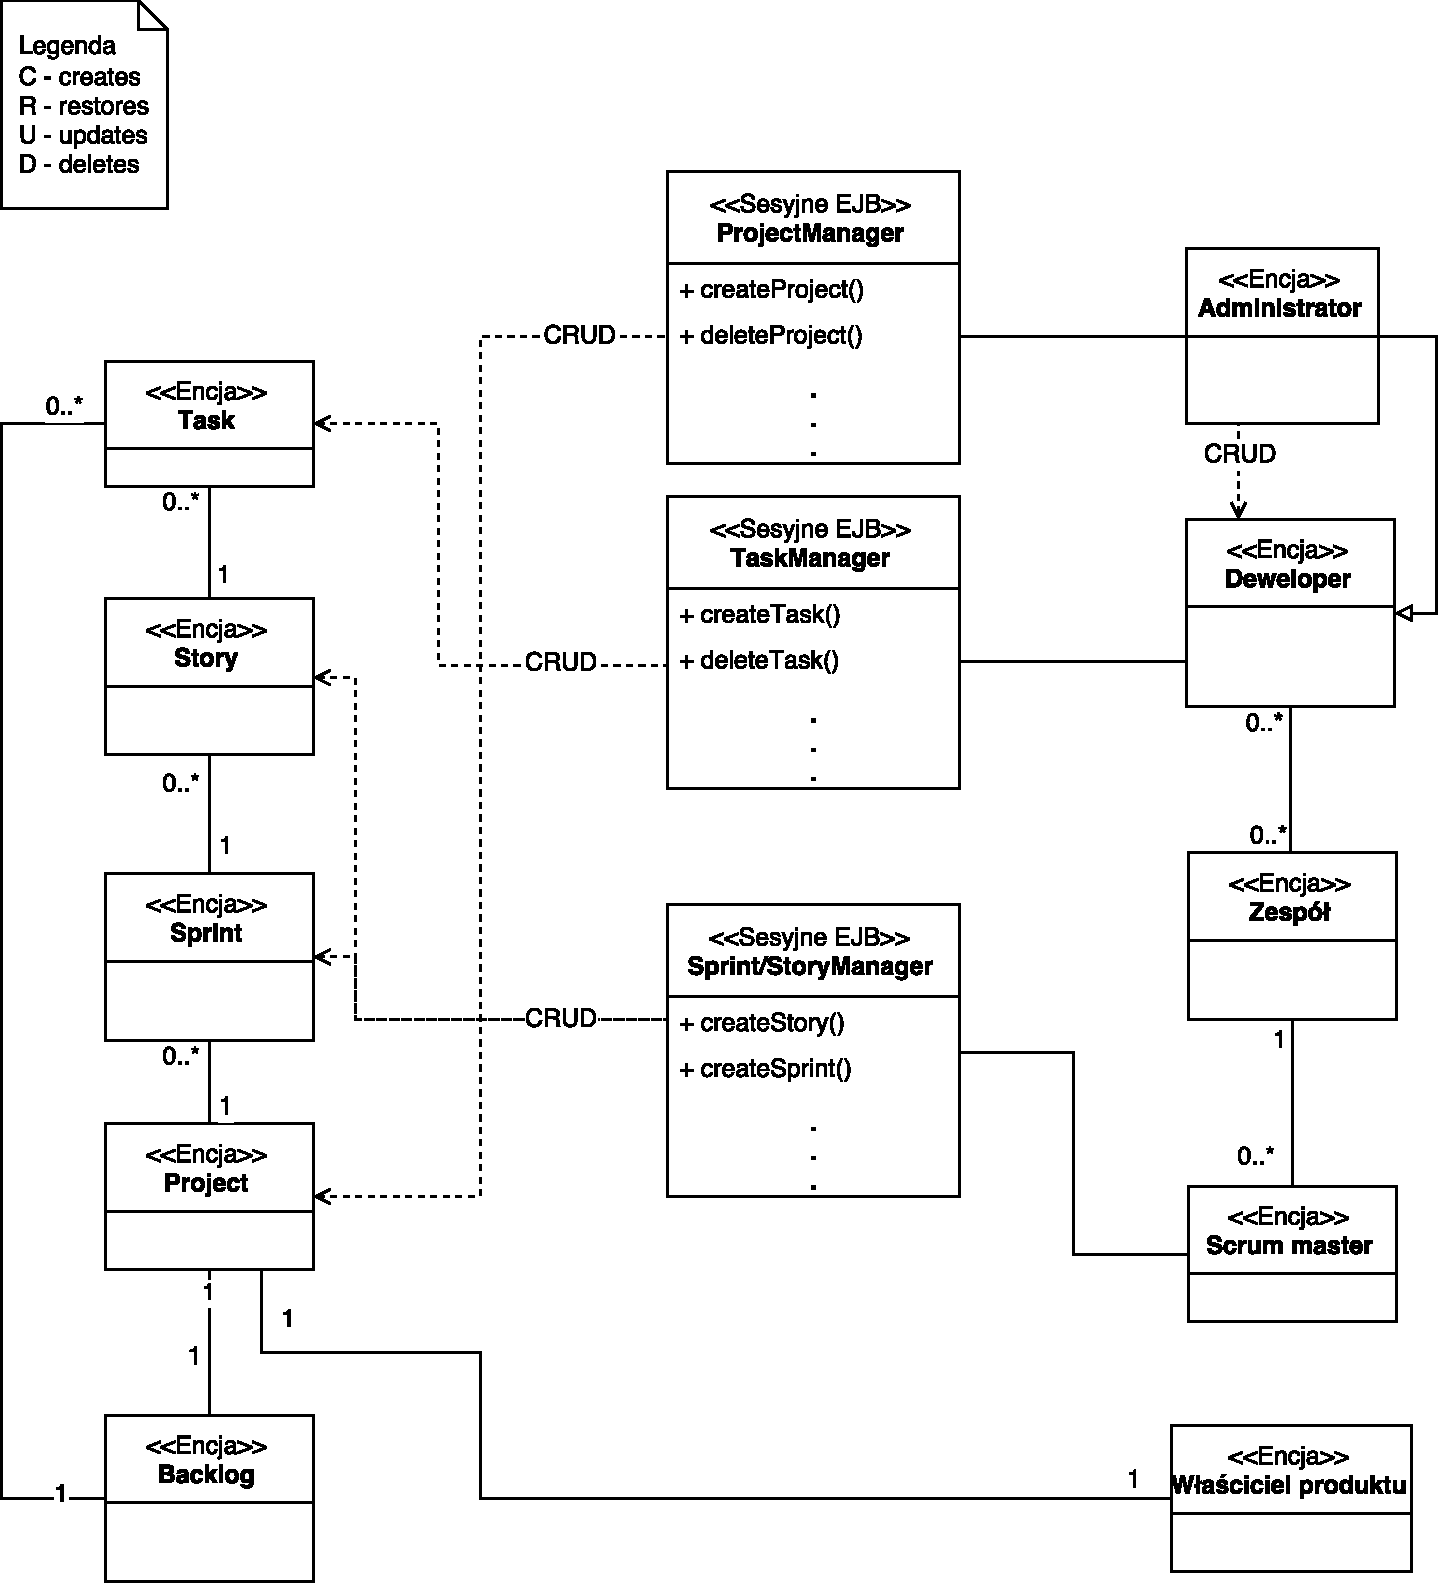
\includegraphics[width=15cm]{rysunki/diagdetailuml.pdf}	
	\caption{Szczegółowy diagram wybranych klas}
	\label{fig:diagdetailuml}
\end{figure}

\subsection{Klasyfikacja komponentów EJB}
W tej sekcji zostaną opisane komponenty EJB używane w aplikacji oraz takie, które nie zostały użyte wraz z podaniem argumentów dlaczego je pominięto.

\subsubsection{Komponenty encyjne}
Reprezentują rekordy utrwalone w bazie danych. Komponenty encyjne mogą być używane do reprezentowania rzeczowników lub rzeczy z opisu funkcjonalnego. Jeżeli jednostka biznesowa posiada odpowiednik w rzeczywistości, to jest to prawdopodobnie komponent encyjny.

\subsubsection{Komponenty sesyjne}
Podczas gdy komponenty encyjne są rzeczami w aplikacji, komponenty sesyjne określają czynności jakie można na tych rzeczach wykonać. Są one jednostkami kontrolującymi procesy biznesowe. Zatem, aby wyodrębnić ten rodzaj komponentów należy się skupić na tym, co aplikacja może robić.
Przyglądając się diagramowi klas można zauważyć, że ProjectManager może wykonywać operacje Create Restore Update Delete (CRUD) na projektach.
Gdy w dowolnej aplikacji funkcjonalności skupiają się zazwyczaj wokół jednej lub więcej encji, to znaczy, że prawdopodobnie jest to komponent sesyjny. Ta reguła również tutaj ma swoje zastosowanie. Zostały utworzone odpowiednie komponenty sesyjne, które są swego rodzaju menedżerami spinającym funkcjonalności biznesowe, które są ze sobą powiązane. Ponieważ komponent sesyjny definiuje zbiór zachowań, to każde takie zachowanie można podporządkować jednej metodzie.

Głównym zadaniem aplikacji będzie przeglądanie projektów oraz zadań. W tym celu zostały utworzone odpowiednie komponenty sesyjne dla każdego rodzaju obiektu biznesowego, które jednak nie zostały przedstawione na szczegółowym diagramie, ze względu na ich obszerność. Każdy taki komponent posiada metody CRUD, które umożliwiają wykonywanie dowolnych operacji na tychże obiektach.

Tworzona aplikacja skupia się na zarządzaniu projektami, więc bez konfiguracji wstępnej – utworzenia użytkowników, przyznanie praw właściciela produktu, czy administratora  – zarządzanie, a nawet samo utworzenie projektu będzie nie możliwe. Ponieważ tymi rzeczami zajmuje się administrator, więc w działającym systemie musi istnieć już użytkownik z uprawnieniami administratora. Dzięki temu system jest gotowy do działania zaraz po uruchomieniu.

\subsubsection{Komponenty sterowane komunikatami}
Pomimo iż zostało postanowione, że w aplikacji nie będą użyte komponenty sterowane komunikatami, nic nie stoi na przeszkodzie, aby głębiej przemyśleć możliwość wykorzystania takich komponentów. Zastanówmy się, w jakich sytuacjach mogłyby one być korzystne.

Pierwszą rzeczą, która nasuwa się na myśl jest wykorzystanie MDB (Message Driven Bean) do generowania i wysyłania e-maili z hasłem po utworzeniu użytkownika. Taka wiadomość mogła by być rozgłoszona w systemie i dzięki temu różne komponenty mogłyby obsłużyć to zdarzenie. W systemie zrezygnowano jednak z tego typu technik.

Drugim możliwym zastosowaniem jest możliwość wysyłania rozgłoszeń w systemie. Jednak że aplikacja nie wprowadza funkcjonalności wiadomości systemowych również i tu ten komponent nie ma zastosowania.

Na tym etapie warto wspomnieć, że komponenty sterowane komunikatami można wprowadzić na każdym etapie udoskonalania projektu jednak warto zwrócić uwagę na to, jak zachować odpowiedni stopień bezpieczeństwa przy tego typu komunikatach.

\section{Model bazy danych}
System korzysta z zewnętrznej bazy danych, której model jest przedstawiony na rysunku \ref{fig:modeldb}. Został on wygenerowany za pomocą testowej wersji programu DbSchema. Kolorem zielonym zostały oznaczone tabele dotyczące użytkowników oraz uprawnień. Niebieski kolor oznacza tabele złączeniowe, które nie mają odwzorowania w kodzie. Czerwone zaś to pozostałe struktury występujące w projekcie -- są to obiekty na których operują użytkownicy. W pozostałej części pracy opiszę jak został wygenerowany model bazy danych.

\begin{sidewaysfigure}[h!]
	\centering
	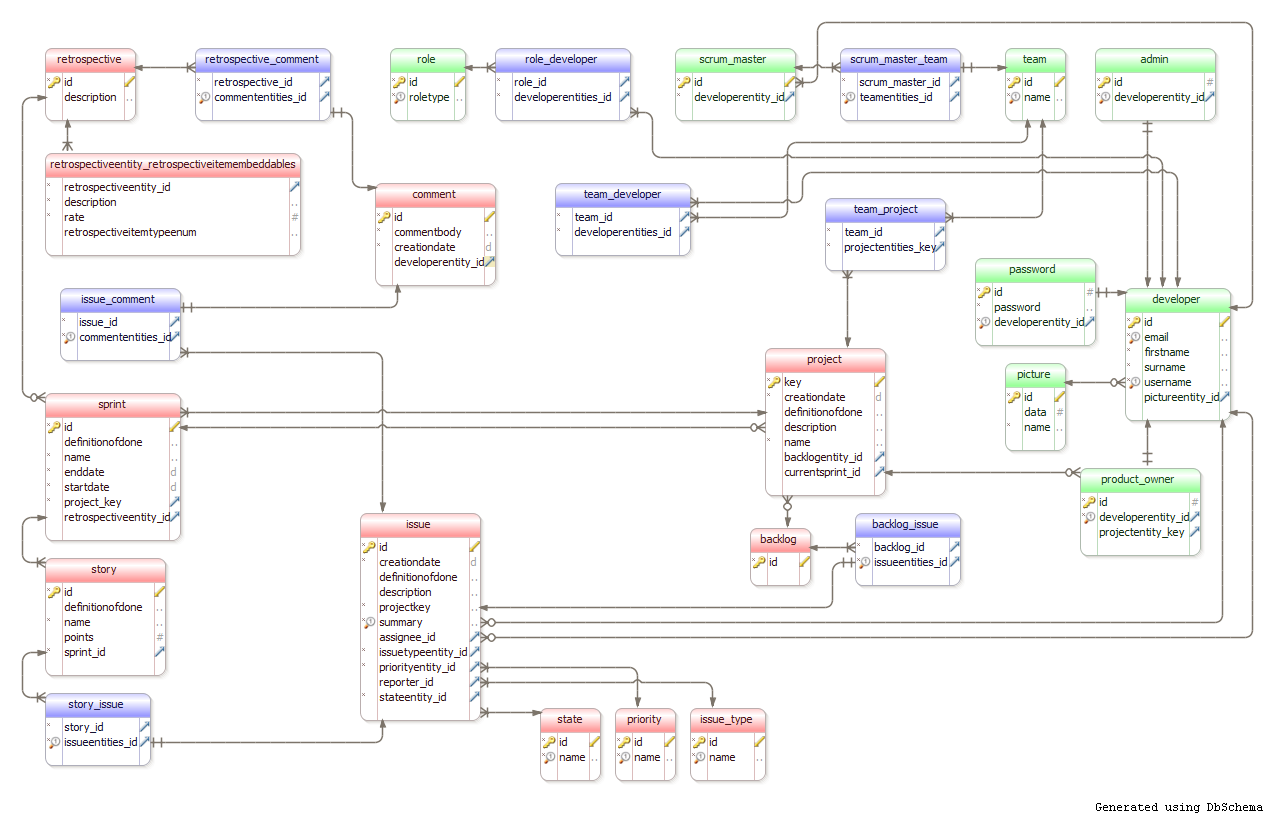
\includegraphics[width=25cm]{rysunki/modeldb.png}	
	\caption{Szczegółowy diagram wybranych klas}
	\label{fig:modeldb}
\end{sidewaysfigure}
\chapter{Dokumentacja projektowa}

\section{Architektura systemu}
Wytworzony przeze mnie system jest aplikacją webową, która korzysta z bazy danych do odczytu i zapisu niezbędnych informacji. Z systemu będą korzystać cztery, wcześniej omówione, rodzaje użytkowników poprzez interfejs WWW. Dodatkowo system został zaprojektowany w taki sposób, aby była możliwość rozbudowy o dodatkowe zdalne aplikacje klienckie umożliwiające komunikację z systemem. System wraz z bazą danych znajdują się w kontenerze Dockera.

Jak wiadomo, połączenie ze zdalnymi klientami nie jest gwarantowane, co skłania do zastosowania mechanizmu komunikacji Java Message Service (JMS). Jednak pomimo, że połączenie nie jest ani stabilne, ani nawet w ogóle nie wiadomo czy zostało nawiązane, zależy nam, aby informować użytkowników o różnego rodzaju błędach, lub przesyłać im dane na bieżąco. Co prawda JMS umożliwia realizację tego zadania lecz do komunikacji z samodzielną aplikacją zostały udostępnione inne ścieżki komunikacji. 

Pierwsza z nich to warstwa usługi REST. Dzięki takiemu rozwiązaniu z aplikacją może komunikować się dowolny system niezależnie od tego w jakim języku został napisany. Warstwa ta nie została zaimplementowana w całości, lecz jedynie w jako fragment funkcjonalności w celu zobrazowania komunikacji ze zdalnymi klientami.

Kolejna ścieżka komunikacji to zdalny interfejs komponentu EJB (Enterprise JavaBean). Mechanizm ten wprowadza możliwość komunikacji asynchronicznej z aplikacją. Jest one jednak ograniczony tylko do klientów napisanych w języku Java.

Wyżej wymienione rozwiązania stanowią warstwę do komunikacji z aplikacjami klienckimi. Kolejnym krokiem było zaprojektowanie warstwy do komunikacji z klientem WWW. Co prawda warstwa REST spełniałaby swoje wymagania, lecz w tym celu posłużymy się, specjalnie zaprojektowaną do tego rodzaju zadań, technologią JavaServer Faces (JSF), która będzie wymagała dodatkowej warstwy z którą będzie się komunikować. Warstwa ta to tzw. komponenty Java Beans zwane również Backing Beans (BB). Rysunek \ref{fig:diagsys} przedstawia diagram systemowy aplikacji:

\begin{figure}[h!]
	\centering
	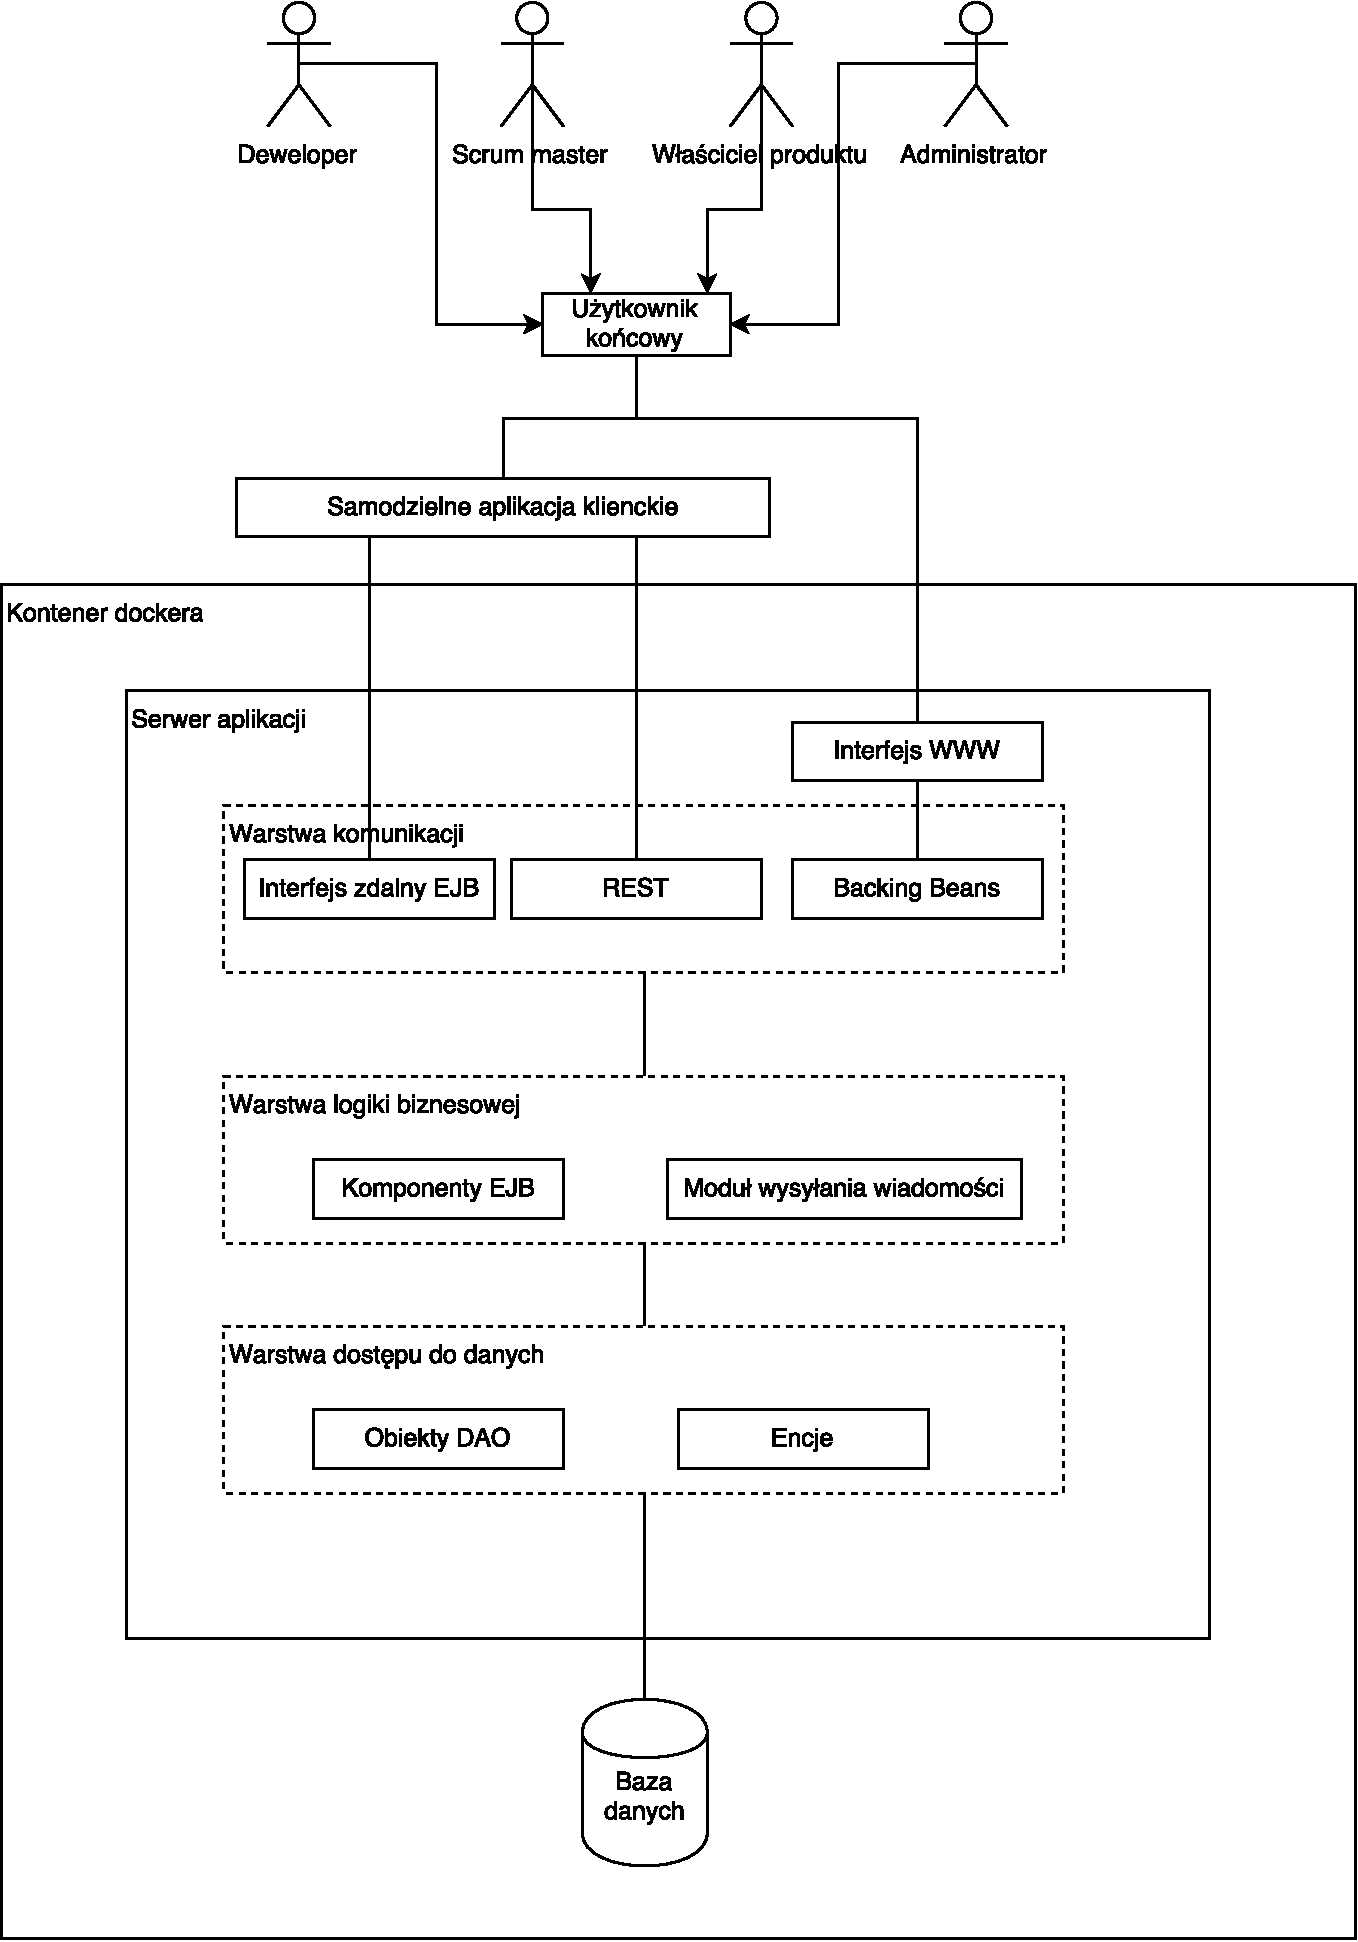
\includegraphics[width=13.5cm]{rysunki/diagsys.pdf}	
	\caption{Diagram systemowy aplikacji}
	\label{fig:diagsys}
\end{figure}

Jak wiadomo, interfejsy graficzne, a co za tym idzie – sposób ich obsługi będą się różniły w zależności od klienta. Najważniejszą różnicą będzie sposób walidacji danych oraz obsługi błędów. W samodzielnej aplikacji klienckiej walidacja danych oraz obsługa błędów powinna wystąpić możliwie szybko, aby nie generować zbędnego ruchu sieciowego. Jeżeli w trakcie przetwarzania żądania wystąpią jakiekolwiek błędy, to powinny one zostać zamienione na wyjątki aplikacji oraz przekazane do klienta. Również w aplikacji WWW walidacja danych wejściowych powinna znajdywać się na poziomie klienta. Jednak nie można wykluczyć sytuacji, w której błędy pojawią się po stronie serwera nawet po poprawnej walidacji danych. Z tego względu błędy powinny być konwertowane po stronie serwera (przez dodatkową warstwę obsługi JSF) na obiekty typu FaceMessage i dodawane bezpośrednio do kontekstu aplikacji WWW. 

Wymagania odnośnie walidacji oraz obsługi błędów mogą skłaniać do wprowadzenia dodatkowej warstwy w architekturze systemu. Nie mniej jednak taka warstwa nie została wprowadzona, gdyż spowodowało by to nadmierny przyrost klas oraz niepotrzebne uogólnienie systemu. Zamiast tego logika biznesowa generuje wyjątki aplikacji, gdy zajdzie taka potrzeba oraz przekazuje je warstwie wyżej lub klientom, które wywołują dane komponenty logiki biznesowej. Oznacza to tyle, że obsługa błędów aplikacji w samodzielnej aplikacji Javy powinna być zaimplementowana po stronie samej aplikacji, natomiast interfejs WWW posiada dodatkową warstwę w postaci komponentów JavaBeans, które takową obsługę zapewnią. Aby zrozumieć taką modyfikację należy wykonać bardziej szczegółowy diagram systemu. Rysunek 3 przedstawia zmodyfikowany diagram systemu.

\subsection{Identyfikacja komponentów biznesowych}
W oparciu o artefakty metodyki Scrum oraz wymagania funkcjonalne z systemu wyłaniają się następujące komponenty biznesowe:

\textit{Deweloper} -- użytkownik aplikacji, może przeglądać oraz modyfikować \textit{zadania} w \textit{projektach}, do których należy.

\textit{Scrum master} -- użytkownik aplikacji, jest przypisany do jednego lub wielu \textit{zespołów}.

\textit{Właściciel produktu} -- użytkownik aplikacji, jest przypisany tylko do jednego \textit{projektu}.

\textit{Administrator} -- użytkownik aplikacji, zarządza całym systemem. Może tworzyć nowe \textit{projekty} oraz \textit{zespoły}.

\textit{Zespół} -- zbiór \textit{deweloperów}, może być powiązany z \textit{projektem}.

\textit{Projekt} -- zbiór \textit{zadań}, posiada \textit{właściciela produktu}.

\textit{Sprint} -- jest tworzone przez  \textit{scrum mastera}. Posiada story.

\textit{Story} -- jest agregatem \textit{zadań}.

\textit{Backlog} -- przynależy do \textit{projektu}, posiada \textit{zadania}.

\textit{Zadanie} -- jest tworzone przez \textit{użytkowników}.


Należy wspomnień, iż jest to częściowy opis obiektów biznesowych, który ma na celu zobrazowanie procesu powstawania aplikacji. Wyczerpujący opis tych obiektów byłby zbyt rozległy i nie jest on meritum części opisowej pracy. Aby zobrazować wpływ poszczególnych jednostek biznesowych oraz ich wzajemne relacje należy przedstawić ich diagram UML:
\begin{figure}[h!]
	\centering
	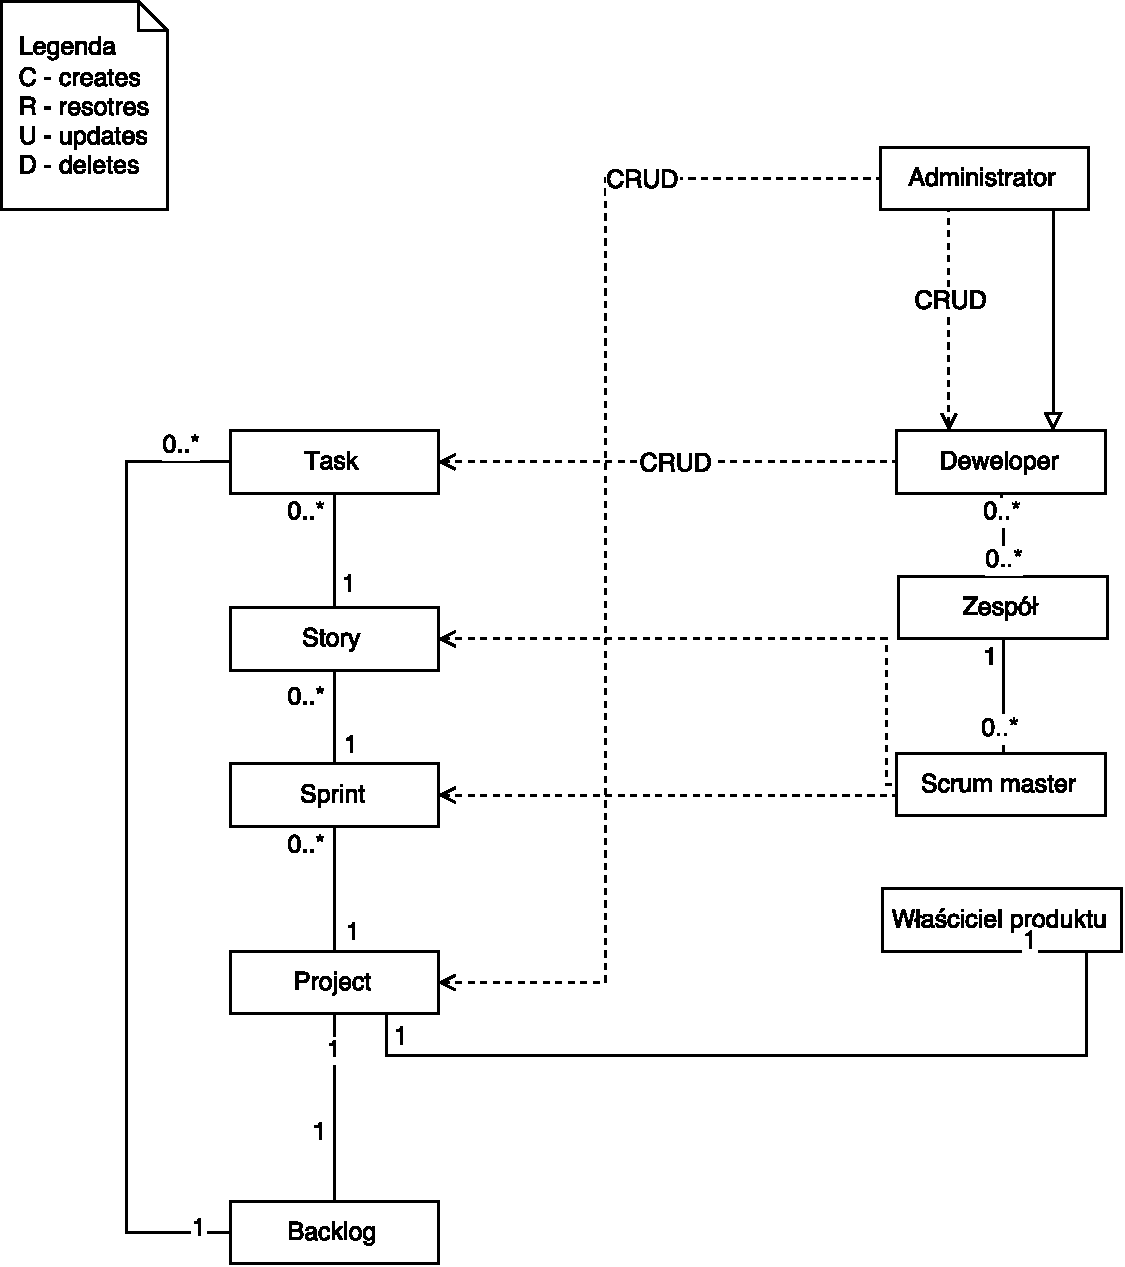
\includegraphics[width=15cm]{rysunki/diaguml.pdf}	
	\caption{Diagram jednostek biznesowych}
	\label{fig:diaguml}
\end{figure}

\section{Struktura projektu}
W poprzedniej sekcji została opisana ogólna architektura systemu umożliwiająca pogląd na całą aplikację. Teraz zostaną opisane wybrane komponenty. Zanim jednak to zrobimy zostanie przedstawiony bardziej szczegółowy diagram jednostek biznesowych, który uwzględnia funkcje, jakie można wykonywać w systemie. Diagram powstał w oparciu o wymagania funkcjonalne, które szczegółowo opisują, co dany użytkownik może robić, oraz o identyfikację komponentów biznesowych omówionych wcześniej. Także i tutaj należy zwrócić uwagę, iż nie jest to wyczerpujący diagram klas opracowanych w systemie:
\begin{figure}[h!]
	\centering
	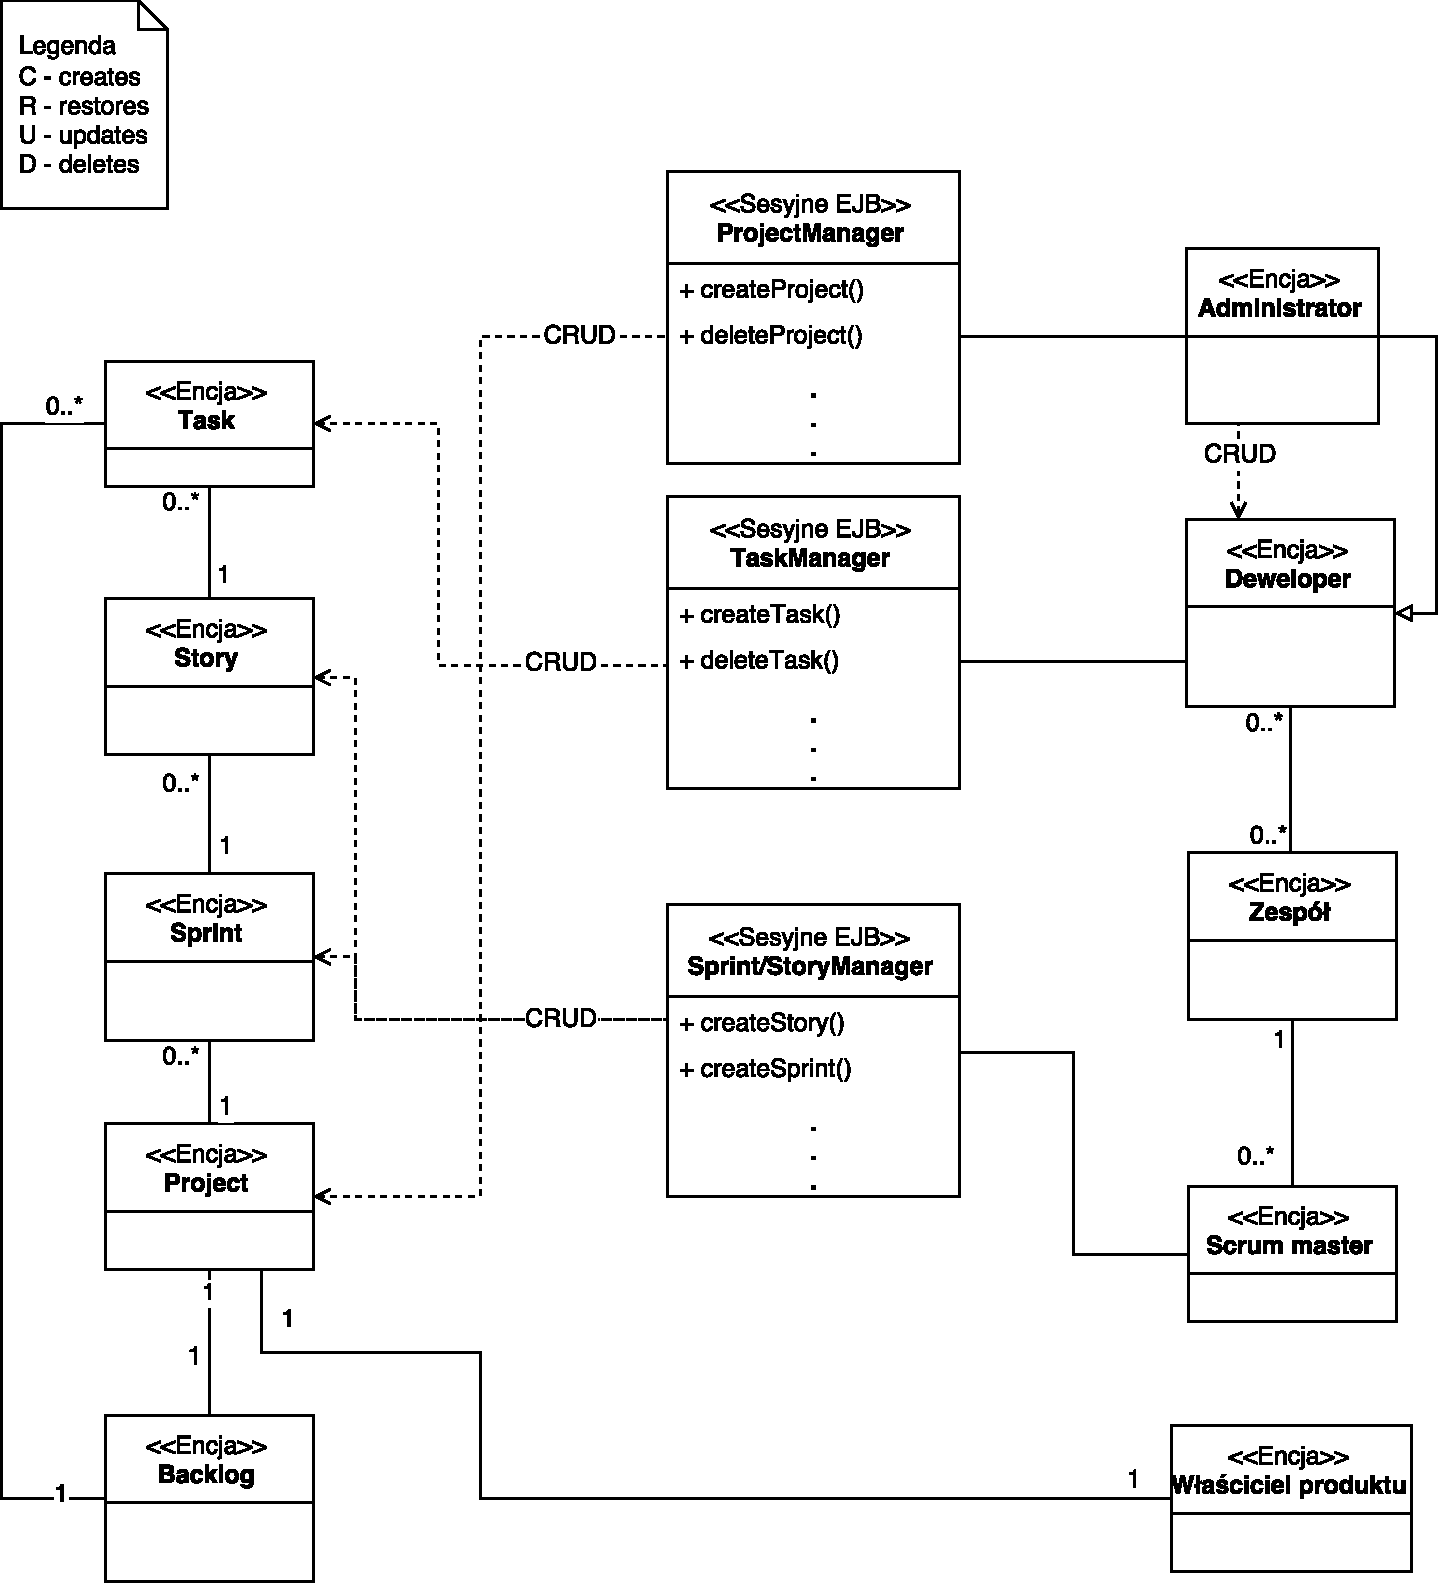
\includegraphics[width=15cm]{rysunki/diagdetailuml.pdf}	
	\caption{Szczegółowy diagram wybranych klas}
	\label{fig:diagdetailuml}
\end{figure}

\subsection{Klasyfikacja komponentów EJB}
W tej sekcji zostaną opisane komponenty EJB używane w aplikacji oraz takie, które nie zostały użyte wraz z podaniem argumentów dlaczego je pominięto.

\subsubsection{Komponenty encyjne}
Reprezentują rekordy utrwalone w bazie danych. Komponenty encyjne mogą być używane do reprezentowania rzeczowników lub rzeczy z opisu funkcjonalnego. Jeżeli jednostka biznesowa posiada odpowiednik w rzeczywistości, to jest to prawdopodobnie komponent encyjny.

\subsubsection{Komponenty sesyjne}
Podczas gdy komponenty encyjne są rzeczami w aplikacji, komponenty sesyjne określają czynności jakie można na tych rzeczach wykonać. Są one jednostkami kontrolującymi procesy biznesowe. Zatem, aby wyodrębnić ten rodzaj komponentów należy się skupić na tym, co aplikacja może robić.
Przyglądając się diagramowi klas można zauważyć, że ProjectManager może wykonywać operacje Create Restore Update Delete (CRUD) na projektach.
Gdy w dowolnej aplikacji funkcjonalności skupiają się zazwyczaj wokół jednej lub więcej encji, to znaczy, że prawdopodobnie jest to komponent sesyjne. Ta reguła również tutaj ma swoje zastosowanie. Zostały utworzone odpowiednie komponenty sesyjne, które są rodzaju menadżerem spinającym funkcjonalności biznesowe, które są ze sobą powiązane. Ponieważ komponent sesyjny definiuje zbiór zachowań, to każde takie zachowanie można podporządkować jednej metodzie.

Głównym zadaniem aplikacji będzie przeglądanie projektów oraz zadań. W tym celu zostały utworzone odpowiednie komponenty sesyjne dla każdego rodzaju obiektu biznesowego, które jednak nie zostały przedstawione na szczegółowym diagramie, ze względu na ich obszerność. Każdy taki komponent posiada metody CRUD, które umożliwiają wykonywanie dowolnych operacji na tychże obiektach.

Tworzona aplikacja skupia się na zarządzaniu projektami, więc bez konfiguracji wstępnej – utworzenia użytkowników, przyznanie praw właściciela produktu, czy administratora  – zarządzanie, a nawet samo utworzenie projektu będzie nie możliwe. Ponieważ tymi rzeczami zajmuje się administrator, więc w działającym systemie musi istnieć już użytkownik z uprawnieniami administratora. Dzięki temu system jest gotowy do działania zaraz po uruchomieniu.

\subsubsection{Komponenty sterowane komunikatami}
Pomimo iż zostało postanowione, że w aplikacji nie będą użyte komponenty sterowane komunikatami, nic nie stoi na przeszkodzie, aby głębiej przemyśleć możliwość wykorzystania takich komponentów. Zastanówmy się, w jakich sytuacjach mogłyby one być korzystne.

Pierwszą rzeczą, która nasuwa się na myśl jest wykorzystanie MDB (Message Driven Bean) generowania i wysyłania e-maili z hasłem po utworzeniu użytkownika. Taka wiadomość mogła by być rozgłoszona w systemie i dzięki temu różne komponenty mogłyby obsłużyć to zdarzenie. W systemie zrezygnowano jednak z tego typu technik.

Drugim możliwym zastosowaniem jest możliwość wysyłania rozgłoszeń w systemie. Jednak że aplikacja nie wprowadza funkcjonalności wiadomości systemowych również i tu ten komponent nie ma zastosowania.

Na tym etapie warto wspomnieć, że komponenty sterowane komunikatami można wprowadzić na każdym etapie udoskonalania projektu jednak warto zwrócić uwagę na to, jak zachować odpowiedni stopień bezpieczeństwa przy tego typu komunikatach.
\chapter{Podsumowanie}

\section{Przegląd projektu}
W trakcie pracy nad systemem wykorzystano wiele nowych technologii, które przyczyniły się do jego jakości oraz stabilności. Pierwszym celem jaki został postawiony systemowi była jego użyteczność -- zostały zaimplementowane tylko obligatoryjne funkcje systemu, jaki powinien posiadać projekt tej kategorii. W łatwy i przejrzysty sposób pozwala on zarządzać projektem, który jest prowadzony za pomocą metodyki Scrum. 

Następnie w celu zapewnienia trwałości wszystkie dane systemu zapisywane są w darmowej i popularnej bazie Postgres. Przy procesie interakcji z bazą posłużyła nam specyfikacja JPA oraz jej implementacja oparta na Hibernate. Takie rozwiązanie sprawia, że modyfikacja i pielęgnacja już istniejącego kodu nie powinna sprawiać żadnych problemów.

Do osiągnięcia kolejnego celu pracy - przejrzystości interfejsu użytkownika - zastosowano dobrze znany i lubiany framework JSF wzbogacony o darmowe komponenty z biblioteki Primefaces. Umożliwiło to skupienie się na wytwarzaniu funkcjonalności systemu zapewniając jednocześnie jego prostotę i elegancję.

Ostatnim celem była prosta konfiguracja i zarządzanie systemem oraz szybka reakcja na niedostępność systemu. Został on osiągnięty dzięki wykorzystaniu systemu Docker, który jest pionierem jeżeli chodzi o szybie wytwarzanie i uruchamianie środowisk zarówno deweloperskich jak i testowych. 

Całość została uzupełniona o testy jednostkowe oraz integracyjne. W kodzie wykorzystano szereg udogodnień, jakie wprowadza wersja ósma Javy. Dodatkowo praktyczna znajomość wzorców projektowych pozwoliła na efektywniejszą pracę i szybszą implementację funkcjonalności przy jak najmniejszym wysiłku.


\section{Czy można było zrobić coś lepiej?}
Oczywiście, jak każdy projekt informatyczny, tak i ten posiada pewne wady. Został on napisany jako monolityczna aplikacja webowa, co sprawia, że wgranie nowej funkcjonalności powoduje konieczność ponownego wdrożenia całego systemu.

System może zostać zrefaktoryzowany do postaci szeregu mikroserwisów, z których każdy posiada swoją odpowiedzialność. Na przykład serwis użytkowników odpowiadający za autentykację i autoryzację, serwis warstwy prezentacji korzystający z serwisu danych np. zadań lub projektów. Całość mogłaby również zostać oparta na Dockerach oraz na technologi mikroserwisów, którą wspaniale wspierają takie projekty jak SpringBoot.

Aktualna implementacja systemu również sprawia, że jest on przejrzysty, prosty w konfiguracji oraz estetycznie wyglądający. Są to najważniejsze cechy takich projektów, które mogą przyciągnąć uwagę wielu potencjalnych użytkowników.
\chapter{Literatura}
\begin{thebibliography}{99}
	\bibitem{JSF} JavaServer Faces i Eclipse Galileo. Tworzenie aplikacji WWW \emph{Andrzej Marciniak} Helion 2010
	\bibitem{JSF_CORE} Core JavaServer Faces. Wydanie II \emph{David Geary, Cay S. Horstmann} Helion 2008
	\bibitem{EJB_3.0} Enterprise JavaBeans 3.0 \emph{Bill Burke \& Richard Monson-Haefel} Helion 2007
	\bibitem{JBOSS_7} JBoss AS 7. Tworzenie aplikacji \emph{Francesco Marchioni} Helion 2014
	\bibitem{J2EE} Core J2EE. Wzorce projektowe \emph{Deepak Alur, John Crupi, Dan Malks} Helion 2004
	\bibitem{SCRUM} Scrum. O zwinnym zarządzaniu projektami. Wydanie II rozszerzone \emph{Mariusz Chrapko} Helion 2015
	\bibitem{JAVA} Java. Kompedium programisty. Wydanie VIII \emph{Herbert Schildt} Helion 2012
	\bibitem{CI} Zwinne wytwarzanie oprogramowania. Najlepsze zasady, wzorce i praktyki \emph{Robert C. Martin} Helion 2015
	\bibitem{GIT} Git. Rozproszony system kontroli wersji \emph{Włodzimierz Gajda} Helion 2013
	\bibitem{CLEAN_CODE_MASTER} Mistrz czystego kodu. Kodeks postępowania profesjonalnych programistów \emph{Robert C. Martin} Helion 2013
	\bibitem{CLEAN_CODE} Czysty kod. Podręcznik dobrego programisty \emph{Robert C. Martin} Helion 2010
	\bibitem{WZORCE} Rusz głową! Wzorce projektowe \emph{Eric Freeman, Elisabeth Freeman, Bert Bates, Kathy Sierra} Helion 2011
	\bibitem{REFACTOR} Refaktoryzacja do wzorców projektowych \emph{Joshua Kerievsky} Helion 2005	
\end{thebibliography}
	

\end{document}